% This is LLNCS.DEM the demonstration file of
% the LaTeX macro package from Springer-Verlag
% for Lecture Notes in Computer Science,
% version 2.4 for LaTeX2e as of 16. April 2010
%
\RequirePackage{amsmath,amssymb}
\PassOptionsToPackage{svgnames,dvipsnames,svgnames}{xcolor}
\documentclass{llncs}
%
\usepackage{stmaryrd}
\usepackage{wasysym}
\usepackage{makeidx}  % allows for indexgeneration
\usepackage{mathpartir} % inference rules
\usepackage{extarrows}
\usepackage{graphicx}
\usepackage{url}
\usepackage{xcolor}
\usepackage[bookmarks=true,colorlinks=true,allcolors=Green,breaklinks]{hyperref}
%\usepackage[pdfborder={0 0 0}]{hyperref}
%\usepackage[colorlinks=true,allcolors=Green,backref,pageanchor=true,plainpages=false, pdfpagelabels, bookmarks,bookmarksnumbered,
%pdfborder={0 0 0},  %removes outlines around hyper links in online display
%]{hyperref}

% !TEX root = editor-tfp16.tex

% HTyp and HExp
\newcommand{\hcomplete}[1]{#1~\mathsf{complete}}

% HTyp
\newcommand{\htau}{\dot{\tau}}
\newcommand{\tarr}[2]{#1 \rightarrow #2}
\newcommand{\tnum}{\texttt{num}}
\newcommand{\tehole}{\llparenthesis\rrparenthesis}

\newcommand{\tcompat}[2]{#1 \sim #2}

% HExp
\newcommand{\hexp}{\dot{e}}
\newcommand{\hlam}[3]{\lambda #1{:}#2.#3}
\newcommand{\hap}[2]{#1(#2)}
\newcommand{\hnum}[1]{\underline{#1}}
\newcommand{\hadd}[2]{#1 + #2}
\newcommand{\hehole}{\llparenthesis\rrparenthesis}
\newcommand{\hhole}[1]{\llparenthesis#1\rrparenthesis}

\newcommand{\hGamma}{\dot{\Gamma}}
\newcommand{\domof}[1]{\text{dom}(#1)}
\newcommand{\hsyn}[3]{#1 \vdash #2 \Rightarrow #3}
\newcommand{\hana}[3]{#1 \vdash #2 \Leftarrow #3}

% ZTyp and ZExp
\newcommand{\zlsel}[1]{{\bowtie}{#1}}
\newcommand{\zrsel}[1]{{#1}{\bowtie}}
\newcommand{\zwsel}[1]{{\triangleright}{#1}{\triangleleft}}

\newcommand{\removeSel}[1]{#1^{\diamond}}

% ZTyp
\newcommand{\ztau}{\hat{\tau}}

% ZExp
\newcommand{\zexp}{\hat{e}}

% Direction
\newcommand{\dParent}{\mathtt{parent}}
\newcommand{\dChild}{\mathtt{firstChild}}
\newcommand{\dNext}{\mathtt{nextSib}}
\newcommand{\dPrev}{\mathtt{prevSib}}

% Action
\newcommand{\aMove}[1]{\mathtt{move}~#1}
	\newcommand{\zrightmost}[1]{\mathsf{rightmost}(#1)}
	\newcommand{\zleftmost}[1]{\mathsf{leftmost}(#1)}
\newcommand{\aSelect}[1]{\mathtt{sel}~#1}
\newcommand{\aDel}{\mathtt{del}}
\newcommand{\aReplace}[1]{\mathtt{replace}~#1}
\newcommand{\aConstruct}[1]{\mathtt{construct}~#1}
\newcommand{\aFinish}{\mathtt{finish}}

\newcommand{\performAna}[5]{#1 \vdash #2 \Leftarrow #3 \xlongrightarrow{#4} #5}
\newcommand{\performSyn}[5]{#1 \vdash #2 \Rightarrow #3 \xlongrightarrow{#4} #5}
\newcommand{\performTyp}[3]{#1 \xlongrightarrow{#2} #3}

\newcommand{\performMove}[3]{#1 \xlongrightarrow{#2} #3}
\newcommand{\performDel}[2]{#1 \xlongrightarrow{\aDel} #2}

% Form
\newcommand{\farr}{\mathtt{arr}}
\newcommand{\fnum}{\mathtt{num}}

\newcommand{\fasc}{\mathtt{asc}}
\newcommand{\fvar}[1]{\mathtt{var}~#1}
\newcommand{\flam}[1]{\mathtt{lam}~#1}
\newcommand{\fap}{\mathtt{ap}}
\newcommand{\fnumlit}[1]{\mathtt{numlit}~#1}
\newcommand{\fplus}{\mathtt{plus}}
\newcommand{\fhole}{\mathtt{hole}}

%
\begin{document}

%
\frontmatter          % for the preliminaries

\mainmatter              % start of the contributions
%
\title{Hazelnut: A Bidirectionally Typed \\Structure Editor Calculus}
\subtitle{(Research Paper Draft)}
%
%\titlerunning{Hamiltonian Mechanics}  % abbreviated title (for running head)
%                                     also used for the TOC unless
%                                     \toctitle is used
%
\author{Cyrus Omar\inst{1}$^\dagger$ \and Michael Hilton\inst{2}$^\dagger$ \and
Ian Voysey\inst{1}$^\dagger$ \and \\Jonathan Aldrich\inst{1} \and Matthew A. Hammer\inst{3}}
%
\authorrunning{Omar et al.} % abbreviated author list (for running head)
%
%%%% list of authors for the TOC (use if author list has to be modified)
%\tocauthor{Ivar Ekeland, Roger Temam, Jeffrey Dean, David Grove,
%Craig Chambers, Kim B. Bruce, and Elisa Bertino}
%
\institute{Carnegie Mellon University
%\email{comar@cs.cmu.edu}\\
%\texttt{http://www.cs.cmu.edu/\homedir comar/}
\and
Oregon State University
%\email{hiltonm@eecs.oregonstate.edu}\\
\and
University of Colorado Boulder
%\email{Matthew.Hammer@colorado.edu}
\\
{}$^\dagger$~{Student Author}
}

\maketitle              % typeset the title of the contribution
\begin{abstract}
Programs are rich inductive structures, but  programmers typically construct and manipulate them only indirectly, through flat textual representations. This indirection  comes at a cost -- programmers must comprehend the various subtleties of parsing, and it can require many text editor actions to make a single syntactically and semantically well-defined change. %Manipulating ill-defined programs is difficult for programmers and complicates the design of programming tools.
During these sequences of text editor actions, or when the programmer makes a mistake, programmers and programming tools must contend with malformed or semantically ill-defined program text, complicating the programming process.
%Unfortunately, this fact is somewhat obscure because  programmers typically construct and interact with  programs only indirectly, using a text editor composed with a parser.
%There are some benefits to this approach, to be sure, but the structural mismatch between programs and text  also imposes a cognitive burden.
%For example, the primitive edit actions available in a text editor (e.g. inserting or deleting a character or word)  do not always correspond to  sensible structural transformations.
%Indeed, most structural  transformations require performing many primitive edit actions.

\emph{Structure editors} promise to alleviate these burdens by exposing only edit actions that  produce sensible changes to the program structure.
Existing designs for structure editors, however, are complex and somewhat \emph{ad hoc}. They also focus primarily on syntactic well-formedness, so programs can still be left semantically ill-defined as they are being constructed.

In this paper, we report on our ongoing efforts to develop Hazelnut, a minimal  structure editor defined in a principled type-theoretic style that permits only syntactically and semantically well-defined actions, without forcing the programmer to construct the program in a strictly ``top-down'' fashion.
Formally, Hazelnut is a bidirectionally typed lambda calculus extended with
1) \emph{holes} (which mark subterms that are under construction);
%, which are identified by variables tracked in a separate linear \emph{hole context}
2) a \emph{focus model}; and 3) a bidirectional \emph{action model} equipped with a useful \emph{action sensibility} metatheorem. %Programs with holes have a well-defined static semantics, and the action model is defined such that every performable action is both syntactically sensible (by construction) and semantically sensible (i.e. we can establish a useful \emph{action sensibility} theorem.)
%We conclude by outlining our vision of a full-scale programming system grown ``from the ground up'' around the same fundamental principles as Hazelnut.

%\keywords{computational geometry, graph theory, Hamilton cycles}
\end{abstract}
%
\section{Introduction}
%
% !TEX root = editor-tfp16.tex

%% Programs (and, by the Curry-Howard correspondence, proofs) are rich
%% inductive structures. This fact is well understood amongst researchers
%% and experienced programmers, but still somewhat obscure amongst
%% programmers at large because programmers normally construct and interact
%% with programs only indirectly, e.g. using a text editor composed with a
%% parser.

%% There are some benefits to this approach, to be sure, but the structural
%% mismatch between programs and their textual representations also imposes
%% various burdens.  For example, the primitive edit actions available in a
%% text editor (e.g. inserting or deleting a character or word) do not
%% always correspond to sensible structural transformations.

% spj: describe the problem; state our contributions; STOP. one page max.

% When constructing a program or proof in a language with rich type
% structure, skilled programmers generally follow a \emph{type discipline}
% where they first determine the type of the expression that they are
% constructing in order to constrain the mental search space that they are
% operating within.

% For example, if the programmer knows that an expression of type
% $\tarr{\tnum}{\tnum}$ is needed, then it is often the case (though, of course, not
% necessarily the case) that the expression will take the form $$\hlam{\mathit{x}}{e}$$
% for some variable $x$ and function body $e$. If the programmer chooses this
% form, then after picking a suitable variable name, her focus will be on
% constructing a suitable body, $e$. Following the type discipline, $e$ must
% be of type $\tnum$, and so this process can begin anew.

% The problem is that when using a text
% editor to construct a program, it is easy, and indeed necessary, to deviate from this disciplined process.  Rather, text editors operate on sequences of
% characters (i.e. \emph{text}.) 

%Although all programs can be represented as text, most text does not correspond to a syntactically well-formed and semantically well-defined program. 
Programmers and the tools that they use are often presented with text that does not correspond to a well-defined program. This may be because the programmer is in the midst of a sequence of
text edit actions that leave the program ``temporarily'' malformed or ill-defined, or because the programmer has made a mistake. This complicates the programming process, both because the language definition provides no reasoning principles relevant to such text, and, relatedly, because the editor can no longer provide useful services (e.g. syntax highlighting, or semantics-aware code completion.) %Tool designers often develop \emph{ad hoc} heuristic methods that allow one to 
Source code editors sometimes develop \emph{ad hoc} workarounds for this problem, e.g. they might use whitespace to guess where a construct is likely to end, or recover from a type error by pretending that the type was as expected (if, indeed, an expected type can be determined.)

% stuck editing a representation of the program instead of the structures
% themselves. The editor does not restrict what the programmer may do: you
% can delete characters that belong, insert ones that don't, forget things
% that were needed, and so. There's nothing stopping us from accidentally
% writing $$\lambda \mathit{x:num}.\mathit{(x,x)}$$ even though it's obvious
% that building a pair can't hope to form a natural number.

% The type structure of the language makes this sort of error obvious: it's
% not that you're adding characters that make your program incorrect, or even
% malformed; you're adding characters that can't possibly create a structure
% you want because of the type. Simply put, the primitive operations
% available in text editors do not always correspond to sensible
% transformations on the structure of the program.

\emph{Structure editors} have made some progress toward addressing this
problem by allowing programmers to edit the tree structure of a program
directly. Each edit action leaves the program being constructed in a
structurally well-formed state.\footnote{In addition to eliminating malformed edit states, it is also generally the case that programs can be written more quickly using a structure editor. However, we will not talk about ``edit costs'' here, because we would like to abstract away from details like whether a keyboard or a mouse (or some other input device) is being used.} We give examples of notable structure editors in Sec. \ref{sec:rw}.  

The problem is that it is still possible to leave the program in a semantically meaningless (i.e. undefined) state, because language definitions generally only give meaning to complete, well-typed terms. This makes it difficult for humans and tools to reason about types and binding during the development process.  %More sophisticated semantic reasoning principles thus remain .

%% TODO: some sort of transition that talks about how you still don't have
%% semantic reasoning principles because you can be left in a semantically
%% ill-defined state

In this paper, we present our ongoing work on a minimal structure editor, Hazelnut,  defined in the type-theoretic style (i.e. Hazelnut is a \emph{structure editor calculus}.) In Hazelnut, expressions and types with \emph{holes} have a well-defined static semantics. Edit actions are type-aware and leave the program in both a structurally and semantically well-defined state. In fact, edit actions maintain an even stronger invariant -- when acting on an expression whose type is determined by its surroundings (e.g. an expression in function argument position), only edit actions consistent with that type are permitted (we will formally state this invariant in Sec. \ref{sec:actions}.) This does not imply that programs need to be constructed in a strictly outside-in manner, however, because an expression that has a type that is not yet consistent with its surroundings can temporarily be put into a {hole} that defers consistency analysis until the hole is \emph{finished}.

The remainder of the paper is organized as follows:
\begin{itemize}
  \item We begin with an example to develop the reader's intuitions in Section
    \ref{sec:example}.

  \item We then formally define Hazelnut in Section \ref{sec:hazel} and state the important metatheoretic properties.

  \item In Section \ref{sec:mech}, we describe our ongoing effort to formalize the semantics and metatheory of Hazelnut in Agda.

  \item In Section \ref{sec:impl}, we describe our ongoing effort to implement Hazelnut in a web browser, using a functional reactive model for user interaction.
  \item In Section \ref{sec:rw}, we give an overview of related work.
  \item We conclude in Section \ref{sec:future} by describing our vision for this work going 
    forward.
\end{itemize}

This paper should be considered a working draft at the time of submission.


\section{Programming in Hazelnut}
\label{sec:example}
\begin{figure}[t]
\[
\begin{array}{|c||c|c||l|l|}
\hline
\# & \textbf{H-Expression} & \textbf{Z-Expression} & \textbf{Next Action} & \textbf{Semantics}
\\
\hline
1 &
\hhole{} &
\zwsel{\hhole{}}
&
\aConstruct{\flam{x}} & \refrule{\ref{r:conelamhole}}
\\ 2 &
\hlam{x}{\hhole{}} : \tarr{\hhole{}}{\hhole{}} &
\hlam{x}{\hhole{}} : \tarr{\zwsel{\hhole{}}}{\hhole{}}
&
\aConstruct{\fnum{}} & \refrule{\ref{r:contnum}}
\\ 3 &
\hlam{x}{\hhole{}} : \tarr{\tnum{}}{\hhole{}} &
\hlam{x}{\hhole{}} : \tarr{\zwsel{\tnum{}}}{\hhole{}}
&
\aMove{\dNext{}} & \refrule{\ref{r:movenextsib}}
\\ 4 &
&
\hlam{x}{\hhole{}} : \tarr{\tnum}{\zwsel{\hhole{}}}
&
\aConstruct{\fnum{}} & \refrule{\ref{r:contnum}}
\\ 5 &
\hlam{x}{\hhole{}} : \tarr{\tnum{}}{\tnum{}} &
\hlam{x}{\hhole{}} : \tarr{\tnum{}}{\zwsel{\tnum{}}}
&
\aMove{\dParent{}} & \refrule{\ref{r:moveparent}}
\\ 6 &
&
\hlam{x}{\hhole{}} : \zwsel{\tarr{\tnum{}}{\tnum{}}}
&
\aMove{\dPrev{}} & \refrule{\ref{r:moveprevsib}}
\\ 7 &
&
\zwsel{\hlam{x}{\hhole{}}} : \tarr{\tnum{}}{\tnum{}}
&
\aMove{\dChild{}} & \refrule{\ref{r:movefirstchild}}
\\ 8 &
&
\hlam{x}{\zwsel{\hhole{}}} : \tarr{\tnum{}}{\tnum{}}
&
\aConstruct{\fvar{x}} & \refrule{\ref{r:conevar}}
\\ 9 &
\hlam{x}{{x}} : \tarr{\tnum{}}{\tnum{}}
&
\hlam{x}{\zwsel{{x}}} : \tarr{\tnum{}}{\tnum{}}
&
\quad\textrm{---{}---}
&
\quad\textrm{---{}---}
\\
\hline
\hline
10 &
\hhole{} &
\zwsel{\hhole{}}
&
\aConstruct{\fasc} & \refrule{\ref{r:constructasc}}
\\ 
11 &
\hhole{} : \hhole{} &
\hhole{} : \zwsel{ \hhole{}}
&
\aConstruct{\fnum{}} & \refrule{\ref{r:contnum}}
\\
12 &
\hhole{} :\tnum{} &
\hhole{} : \zwsel{\tnum{}}
&
\aMove{\dPrev{}} & \refrule{\ref{r:moveprevsib}}
\\
%13 &
%\hhole{} :\tnum{} &
%\zwsel{\hhole{}} : \tnum{}
%&
%\aMove{\dPrev{}} & \refrule{\ref{r:moveprevsib}}
%\\
13 &
%\hhole{} :\tnum{}
 &
\zwsel{\hhole{}} : \tnum{}
&
\aConstruct{ \fvar{id}} & \refrule{\ref{r:conevar2}}
\\
14 &
\hhole{\textrm{$id$}} : \tnum{} &
\hhole{\zwsel{{\textrm{$id$}}}} : \tnum{}
&
\aConstruct{\fap{}} & \refrule{\ref{r:coneapfn}}
\\
15 &
\hhole{\hap{{{\textrm{$id$}}}}{{\hhole{}}}} : \tnum{}
&
\hhole{\hap{{{\textrm{$id$}}}}{\zwsel{\hhole{}}}} : \tnum{}
&
\aConstruct{\fnumlit{3}} &  \refrule{\ref{r:conenumnum}}
\\
16 &
\hhole{\hap{{{\textrm{$id$}}}}{{\hnum{3}}}} : \tnum{}
&
\hhole{\hap{{{\textrm{$id$}}}}{\zwsel{\hnum{3}}}} : \tnum{}
&
\aMove{\dParent{}} &  \refrule{\ref{r:moveparent}}
\\
17 &
%\hhole{\hap{{{\textrm{id}}}}{{\hnum{3}}}} : \tnum{}
&
\hhole{\zwsel{\hap{{{\textrm{$id$}}}}{{\hnum{3}}}}} : \tnum{}
&
\aMove{\dParent{}} &  \refrule{\ref{r:moveparent}}
\\
18 &
%\hhole{\hap{{{\textrm{id}}}}{{\hnum{3}}}} : \tnum{}
&
\zwsel{\hhole{{\hap{{{\textrm{$id$}}}}{{\hnum{3}}}}}} : \tnum{}
&
\aFinish &  \refrule{\ref{r:finishana}}
\\
19 &
{\hap{{{\textrm{$id$}}}}{{\hnum{3}}}} : \tnum{}
&
\zwsel{{{\hap{{{\textrm{$id$}}}}{{\hnum{3}}}}}} : \tnum{}
&
\quad\textrm{---{}---} & \quad\textrm{---{}---}
\\
\hline

%% 11 &
%% {\textrm{id}} : \tarr{\tnum{}}{\tnum{}}
%% &
%% \hlam{x}{\zwsel{{x}}} : \tarr{\tnum{}}{\tnum{}}
%% &
%% \aMove{\dParent{}} & ?
%% \\ 12 &
%% %{\textrm{id}} : \tarr{\tnum{}}{\tnum{}}
%% &
%% \zwsel{\hlam{x}{{{x}}}} : \tarr{\tnum{}}{\tnum{}}
%% &
%% \aMove{\dParent{}} & \refrule{15b} bad
%% \\ 13 &
%% %{\textrm{id}} : \tarr{\tnum{}}{\tnum{}}
%% &
%% \zwsel{\hlam{x}{{{x}}} : \tarr{\tnum{}}{\tnum{}}}
%% &
%% \aConstruct{\fap{}} & \refrule{20h} bad
%% \\ 14 &
%% \hapP{{\textrm{id}} : \tarr{\tnum{}}{\tnum{}}}{\hhole{}}
%% &
%% \hapP{{\textrm{id}} : \tarr{\tnum{}}{\tnum{}}}{\zwsel{\hhole{}}}
%% &
%% \aConstruct{\fnumlit{3}} & \refrule{20l} bad
%% \\ 15 &
%% %\hapP{{\textrm{id}} : \tarr{\tnum{}}{\tnum{}}}{\hhole{3}}
%% %&
%% %\hapP{{\textrm{id}} : \tarr{\tnum{}}{\tnum{}}}{\zwsel{\hhole{3}}}
%% %&
%% %\aFinish{} & ?
%% %\\
%% \hapP{{\textrm{id}} : \tarr{\tnum{}}{\tnum{}}}{{\hnum{3}}}
%% &
%% \hapP{{\textrm{id}} : \tarr{\tnum{}}{\tnum{}}}{\zwsel{{\hnum{3}}}}
%% &
%% \quad\textrm{---{}---}
%% &
%% \quad\textrm{---{}---}
%% \\
%% \hline
\end{array}
\]
\caption{Constructing an identity function in Hazelnut (Lines~1--9), then  applying this function (assumed bound to $id$, not shown) to an argument~(Lines 10--19). The formal syntax and referenced rules in the final column are described in Section \ref{sec:hazel}.}
\label{fig:first-example}
\end{figure}
%
Figure~\ref{fig:first-example} gives an example of the Hazelnut user
performing two programming tasks. 
The syntax used in this figure will be formally defined in Section \ref{sec:hazel} -- for now, we will give only the intuitions. In the first task (Lines 1-9), the user constructs the identity function over numbers. In the second task (Lines 10-19), the user applies this function (assumed to be bound to a variable, $id$), to the number expression $\hnum{3}$. 
Each of these tasks is carried out interactively, through the sequence of \emph{actions} shown in the fourth column. 

The second and third columns of the
table show the program as it is being constructed in two forms. The second column shows it as an H-expression, which is an expression that can contain \emph{holes}, delimited by $\llparenthesis$ and $\rrparenthesis$. Z-expressions
are H-expressions with a single focus on some sub-term, indicated by $\triangleright$ and $\triangleleft$. The focus need not be on a hole. 
% on working on filling just one of the holes. 
Each action produces a new Z-expression, which may or may not correspond to a new H-expression.
% to the hole in
%focus in the Z-Expression to produce the next line, which may or may not
%produce a substantively different H-Expression.

Line~1 begins with the simplest initial program: an H-expression 
consisting of a single hole. The corresponding Z-Expression has that hole in focus,
indicated by the syntax~$\zwsel{\hehole}$. Focus determines the locus of action. The first action the user performs is $\aConstruct{\flam{x}}$, which replaces the hole with a lambda abstraction binding the variable $x$. This results in the program on line
2, consisting of a lambda abstraction ascribed an arrow type with holes in all positions and the argument type hole in focus. The
user then proceeds to fill these holes, moving the focus between holes as needed, resulting in the final expression on Line 9. With no holes remaining, this expression is \emph{complete}.% (though it could, of course, undergo further actions nevertheless.)

So far, this development has been type-directed. The user first specified the type of the function, then immediately produced a body of that type on Line 8. Lines 10-12 also begin in a type-directed manner with the user giving an explicit type ascription, indicating that the expression that they are constructing will have type $\tnum$. However, on Line 13, the user performs the $\aConstruct{\fvar{id}}$ action. Recall that $id$ has type $\tarr{\tnum}{\tnum}$, which is not consistent with the type $\tnum$ given in the ascription. Normally, this would produce a type error, leaving the program in a well-formed but semantically undefined state. To avoid this, Hazelnut has two options. One is to simply not make this action available in the program configuration on Line 12. This is inflexible, requiring a top-down approach to program construction (i.e. the user would need to construct the function application form before mentioning $id$.) Instead, Hazelnut permits this action, but places the variable $id$ inside a hole. This defers the consistency check that would normally occur -- a hole can be checked against any type, as long as its contents have some type. The cursor is placed inside the hole. The user then proceeds to apply $id$ to the number expression $\hnum{3}$. At this point, the expression inside the hole has a type consistent with the ascription, so the user can \emph{finish} the hole. In our simple formalism, this requires moving the cursor to the hole (in practice, the system would find the nearest parent of hole form.) The result is a complete, well-typed program on Line 19.

%% The third column~(\textbf{Next Action}) lists the first user action:
%% Constructing a lambda abstraction using variable~$x$.
%% %
%% The final column~(\textbf{Semantics}) indicates the semantic rule for this
%% action, Rule (\ref{r:conelamhole}), which gives general semantics for
%% introducing lambda terms into holes.
%% %
%% In Section~\ref{sec:hazel}, we list this rule, and the other rules used in
%% this final column. In total, these rules give a formal semantics to the
%% user actions, which relate each line's Z-Expression to the Z-Expression on
%% the subsequent line.

%% In addition to introducing the lambda term, and its variable, the
%% first user action~$\aConstruct{\flam{x}}$ also introduces a type
%% ascription for this function, as an arrow type, with holes for the
%% type of its domain and codomain.
%% %
%% The actions for Lines~2--5 consist of the user filling these holes
%% with the basetype $\tnum{}$.
%% %
%% To do so, the user constructs the type constructor twice (Lines 2 and
%% 4), and navigates between the holes with a move action (Line~3).
%% %
%% Generally, the move action~$\dNext$ moves the focus from one
%% sub-structure to the next sibling sub-structure of the (common) parent
%% structure; in this case, it moves from the domain type of the arrow
%% type to the codomain of the arrow type.
%% %


\section{Hazelnut, Formally}
\label{sec:hazel}
Hazelnut is based on the simply-typed lambda calculus extended with a single base type, $\tnum$. Its major constituents, introduced by example in the previous section, are:
\begin{itemize}
\item \textbf{H-types} and \textbf{H-expressions} (Sec. \ref{sec:holes}), which are terms with \emph{holes}. Holes mark subterms that are ``under construction.'' H-types classify H-expressions according to a {bidirectionally typed} static semantics.
\item \textbf{Z-types} and \textbf{Z-expressions} (Sec. \ref{sec:cursors}), which superimpose a single \emph{focus} onto H-types and H-expressions (using Huet's \emph{zipper pattern} \cite{JFP::Huet1997}.)
\item \textbf{Actions} (Sec. \ref{sec:actions}), which move the focus or modify the subterm in focus.

Whenever an action is performed on a well-typed expression, it produces another well-typed expression in a \emph{sensible} manner -- we define \emph{sensibility} in Sec. \ref{sec:actions} as well.
\end{itemize}

\subsection{Holes}\label{sec:holes}
\begin{figure}[t]
$\arraycolsep=4pt\begin{array}{lllllll}
\mathsf{HTyp} & \tau,\htau & ::= &
  \tarr{\htau}{\htau} ~\vert~
  \tnum ~\vert~
  \tehole\\
\mathsf{HExp} & e,\hexp & ::= &
  \hexp : \htau ~\vert~
  x ~\vert~
  \hlam{x}{\hexp} ~\vert~
  \hap{\hexp}{\hexp} ~\vert~
  \hnum{n} ~\vert~
  \hadd{\hexp}{\hexp} ~\vert~
  \hehole ~\vert~
  \hhole{\hexp}
\end{array}$
%\textbf{Sort} & & & \textbf{Operational Form} & \textbf{Stylized Form} & \textbf{Description}\\
\caption{Syntax of H-types and H-expressions. Metavariable $x$ ranges over variables and $n$ ranges over numerals.}
\label{fig:hexp-syntax}
\end{figure}

The syntax of H-types and H-expressions is given in Figure \ref{fig:hexp-syntax}. Most forms correspond directly to those of the simply-typed lambda calculus extended with type $\tnum$. The number expression corresponding to the number $n$ is drawn $\hnum{n}$, and for simplicity, we define only a single arithmetic operation, $\hadd{\hexp}{\hexp}$.

In addition to these standard forms, \emph{empty holes} are drawn $\hehole$ and \emph{non-empty H-expression holes} are drawn $\hhole{\hexp}$. %Holes mark subterms that are, notionally, ``under construction.'' We will see what this formally corresponds to in a moment.

We refer to terms that do not contain subterms of hole form as \emph{complete}. Informally, we will use metavariables $\tau$ and $e$ rather than $\htau$ and $\hexp$ for complete H-types and H-expressions, respectively. Formally, we can derive $\hcomplete{\tau}$ when $\tau$ is a complete H-type, and $\hcomplete{e}$ when $e$ is a complete H-expression. We omit the straightforward definitions of these judgements for concision. The dynamics of Hazelnut, which we need not detail here, is defined only  over complete H-expressions (i.e. the user cannot ``run'' an incomplete program.)

The statics of Hazelnut is organized as a \emph{bidirectional type system} \cite{Pierce:2000:LTI:345099.345100}, i.e. around the following mutually defined typing judgements:
\[\arraycolsep=15pt\begin{array}{ll}
%\textbf{Judgement Form} & \textbf{Description}\\
\hsyn{\hGamma}{\hexp}{\htau} & \text{$\hexp$ synthesizes $\htau$}\\
\hana{\hGamma}{\hexp}{\htau} & \text{$\hexp$ analyzes against $\htau$}
\end{array}\]
where typing contexts, $\hGamma$, map each variable $x \in \domof{\hGamma}$ to a hypothesis $x : \htau$.

Algorithmically, the type synthesis judgement specifies a function where the type is an output, and type analysis judgement specifies a function where the type is an input. This defines a \emph{local type inference} scheme, i.e. type ascriptions are unnecessary when an expression is being analyzed against a known type. Moreover, making a judgemental distinction between synthesis and analysis is essential for giving a sensible action semantics to our system (Sec. \ref{sec:actions}.)

 %We use the metavariable $\Gamma$ for \emph{complete typing contexts}, i.e. typing contexts where each hypothesis mentions only complete types.


\begin{subequations}\label{rules:syn-ana}
Type synthesis is stronger than type analysis, i.e. if an expression is able to synthesize a type, it can also be analyzed against that type or any \emph{compatible} type. This is expressed by the following \emph{subsumption rule}:
\begin{equation}\label{rule:ana-subsume}
\inferrule{
  \hsyn{\hGamma}{\hexp}{\htau'}\\
  \tcompat{\htau}{\htau'}
}{
  \hana{\hGamma}{\hexp}{\htau}
}
\end{equation}
The \emph{H-type compatibility} judgement, $\tcompat{\htau}{\htau'}$, reduces to syntactic equality for complete H-types. For incomplete H-types, the rules are given after we discuss the semantics of holes below.

First, let us reproduce the rules for the standard constructs. Type ascription allows the user to explicitly annotate an expression with the type that it is to be analyzed against:
\begin{equation}\label{rule:syn-asc}
\inferrule{
  \hana{\hGamma}{\hexp}{\htau}
}{
  \hsyn{\hGamma}{\hexp : \htau}{\htau}
}
\end{equation}

A variable synthesizes the type that the context assigns to it:
\begin{equation}\label{rule:syn-var}
\inferrule{ }{
  \hsyn{\hGamma, x : \htau}{x}{\htau}
}
\end{equation}

Functions are not themselves annotated with types, so they can only appear in analytic position:
\begin{equation}\label{rule:syn-lam}
\inferrule{
  \hana{\hGamma, x : \htau_1}{\hexp}{\htau_2}
}{
  \hana{\hGamma}{\hlam{x}{\hexp}}{\tarr{\htau_1}{\htau_2}}
}
\end{equation}

For function application, if the expression in function position synthesizes an arrow type, the argument is analyzed against the synthesized argument type:
\begin{equation}\label{rule:syn-ap}
\inferrule{
  \hsyn{\hGamma}{\hexp_1}{\tarr{\htau_2}{\htau}}\\
  \hana{\hGamma}{\hexp_2}{\htau_2}
}{
  \hsyn{\hGamma}{\hap{\hexp_1}{\hexp_2}}{\htau}
}
\end{equation}

Numbers synthesize type $\tnum$:
\begin{equation}\label{rule:syn-num}
\inferrule{ }{
  \hsyn{\hGamma}{\hnum{n}}{\tnum}
}
\end{equation}

Addition operates like a function over numbers:
\begin{equation}\label{rule:syn-plus}
\inferrule{
  \hana{\hGamma}{\hexp_1}{\tnum}\\
  \hana{\hGamma}{\hexp_2}{\tnum}
}{
  \hsyn{\hGamma}{\hadd{\hexp_1}{\hexp_2}}{\tnum}
}
\end{equation}

The rules given so far are sufficient to type complete H-expressions. The remaining rules give H-expressions with holes a well-defined static semantics.

The empty hole synthesizes the hole type:
\begin{equation}\label{rule:syn-ehole}
\inferrule{ }{
  \hsyn{\hGamma}{\hehole}{\tehole}
}
\end{equation}

A non-empty hole contains an H-expression that is ``under construction''. The inner expression must synthesize some type, but the non-empty hole synthesizes only the hole type:
\begin{equation}\label{rule:syn-hole}
\inferrule{
  \hsyn{\hGamma}{\hexp}{\htau}
}{
  \hsyn{\hGamma}{\hhole{\hexp}}{\tehole}
}
\end{equation}
The compatibility judgement $\tcompat{\htau}{\htau'}$, which appeared as a premise in the subsumption rule, makes the hole type compatible with any other type:
\begin{subequations}\label{rules:tcompat}
\begin{equation}\label{rule:tcompat-hole}
\inferrule{ }{
  \tcompat{\htau}{\tehole}
}
\end{equation}
Type compatibility is symmetric and reflexive:
\begin{equation}\label{rule:tcompat-comm}
\inferrule{
  \tcompat{\htau}{\htau'}
}{
  \tcompat{\htau'}{\htau}
}
\end{equation}
\begin{equation}\label{rule:tcompat-num}
\inferrule{ }{
  \tcompat{\tnum}{\tnum}
}
\end{equation}
\begin{equation}\label{rule:tcompat-arr}
\inferrule{
  \tcompat{\htau_1}{\htau_1'}\\
  \tcompat{\htau_2}{\htau_2'}
}{
  \tcompat{\tarr{\htau_1}{\htau_2}}{\tarr{\htau_1'}{\htau_2'}}
}
\end{equation}
\end{subequations}
Consequently, by subsumption, we can derive that $\hana{id : \tarr{\tnum}{\tnum}}{\hhole{id}}{\tnum}$. In other words, the user need not construct the program from the ``outside in''.

The final rule handles function applications where the expression in function position synthesizes a hole type, rather than an arrow type. We treat it as if it had instead synthesized $\tarr{\tehole}{\tehole}$:
\begin{equation}\label{rule:syn-ap-2}
\inferrule{
  \hsyn{\hGamma}{\hexp_1}{\tehole}\\
  \hana{\hGamma}{\hexp_2}{\tehole}
}{
  \hsyn{\hGamma}{\hap{\hexp_1}{\hexp_2}}{\tehole}
}
\end{equation}

The hole type behaves much like the type $?$ in prior work by Siek and Taha on gradual types for functional languages \cite{Siek06a}. Their system (which was not bidirectionally typed nor an editor model) also needed to define two rules for function application. In general, when a premise requires that a synthesized type be of a particular form, we need a special case where the synthesized hole type is treated instead as if it were the ``holey-est'' type of that form.\footnote{Alternatively, we might add a rule that allows expressions that synthesize hole type to then non-deterministically synthesize any other type, but maintaining determinism is useful in practice, so we avoid this approach.}

\end{subequations}
\subsection{Focus Model}\label{sec:cursors}
\begin{figure}[t]
\hspace{-3px}$\arraycolsep=3pt\begin{array}{lllllll}
\mathsf{ZTyp} & \ztau & ::= &
  %\zlsel{\htau} ~\vert~
  \zwsel{\htau} ~\vert~
  %\zrsel{\htau} ~\vert~
  \tarr{\ztau}{\htau} ~\vert~
  \tarr{\htau}{\ztau} \\
\mathsf{ZExp} & \zexp & ::= &
  %\zlsel{\hexp} ~\vert~
  \zwsel{\hexp} ~\vert~
  %\zrsel{\hexp} ~\vert~
  \zexp : \htau ~\vert~
  \hexp : \ztau ~\vert~
  \hlam{x}{\zexp} ~\vert~
  \hap{\zexp}{\hexp} ~\vert~
  \hap{\hexp}{\zexp} ~\vert~
  \hadd{\zexp}{\hexp} ~\vert~
  \hadd{\hexp}{\zexp} ~\vert~
  \hhole{\zexp}
\end{array}$
%\textbf{Sort} & & & \textbf{Operational Form} & \textbf{Stylized Form} & \textbf{Description}\\
\caption{Syntax of Z-types and Z-expressions, i.e. types and expressions with holes and a single cursor.}
\label{fig:zexp-syntax}
\end{figure}

In order to identify a single subtree of an H-type or H-expression as the current focus of action, we apply Huet's \emph{zipper pattern} \cite{JFP::Huet1997}. The syntax of Z-types, $\ztau$, and Z-expressions, $\zexp$, is given in Figure \ref{fig:zexp-syntax}. The only base cases in these inductive grammars are $\zwsel{\htau}$ and $\zwsel{\hexp}$, which identify the H-type or H-expression that is the current focus. All other forms correspond to the recursive forms in the syntax of H-types and H-expressions, and contain exactly one ``hatted'' subterm that identifies the subtree where the focus will be found. All other sub-terms are H-types or H-expressions. Taken together, every syntactically well-formed Z-type and Z-expression contains exactly one focused H-type or H-expression.

We write $\removeSel{\ztau}$ for the H-type constructed by removing the focus marker from the Z-type $\ztau$. This straightforward metafunction is defined as follows:
\begin{align*}
%\removeSel{(\zlsel{\htau})} & = \htau\\
\removeSel{(\zwsel{\htau})} & = \htau\\
%\removeSel{(\zrsel{\htau})} & = \htau\\
\removeSel{(\tarr{\ztau}{\htau})} & = \tarr{\removeSel{\ztau}}{\htau}\\
\removeSel{(\tarr{\htau}{\ztau})} & = \tarr{\htau}{\removeSel{\ztau}}
\end{align*}

Similarly, we write $\removeSel{\zexp}$ for the H-expression constructed by removing the focus marker from the Z-expression $\zexp$:
\begin{align*}
%\removeSel{(\zlsel{\hexp})} & = \hexp\\
\removeSel{(\zwsel{\hexp})} & = \hexp\\
%\removeSel{(\zrsel{\hexp})} & = \hexp\\
\removeSel{(\zexp : \htau)} & = \removeSel{\zexp} : \htau\\
\removeSel{(\hexp : \ztau)} & = \hexp : \removeSel{\ztau}\\
\removeSel{(\hlam{x}{\zexp})} & = \hlam{x}{\removeSel{\zexp}}\\
\removeSel{(\hap{\zexp}{\hexp})} & = \hap{\removeSel{\zexp}}{\hexp}\\
\removeSel{(\hap{\hexp}{\zexp})} & = \hap{\hexp}{\removeSel{\zexp}}\\
\removeSel{(\hadd{\zexp}{\hexp})} & = \hadd{\removeSel{\zexp}}{\hexp}\\
\removeSel{(\hadd{\hexp}{\zexp})} & = \hadd{\hexp}{\removeSel{\zexp}}\\
\removeSel{\hhole{\zexp}} &= \hhole{\removeSel{\zexp}}
\end{align*}

\subsection{Action Semantics}\label{sec:actions}
\begin{figure}[t]
\hspace{-3px}$\arraycolsep=3pt\begin{array}{llcllll}
\mathsf{Action} & \alpha & ::= &
  \aMove{\delta} ~\vert~
  %\aSelect{\delta} ~\vert~
  \aDel ~\vert~
  %\aReplace{\htau} ~\vert~
  %\aReplace{\hexp} ~\vert~
  \aConstruct{\varphi} ~\vert~
  \aFinish\\
\mathsf{Direction} & \delta & ::= &
  \dChild ~\vert~
  \dParent ~\vert~
  \dNext ~\vert~
  \dPrev\\
\mathsf{Form} & \varphi & ::= &
  \farr ~\vert~
  \fnum \\
& & \vert &
  \fasc ~\vert~
  \fvar{x} ~\vert~
  \flam{x} ~\vert~
  \fap ~\vert~
  \farg ~\vert~
  \fnumlit{n} ~\vert~
  \fplus
\end{array}$
%\textbf{Sort} & & & \textbf{Operational Form} & \textbf{Stylized Form} & \textbf{Description}\\
\caption{Syntax of actions.}
\label{fig:action-syntax}
\end{figure}

The syntax of \emph{actions}, $\alpha$, is given in Figure \ref{fig:action-syntax}. Actions can be performed on Z-types and Z-expressions according to the \emph{action semantics} of Hazelnut, which is organized around three judgements:
\[\arraycolsep=10pt\begin{array}{ll}
%\textbf{Judgement Form} & \textbf{Description}\\
\performTyp{\ztau}{\alpha}{\ztau'} & \text{Performing $\alpha$ on $\ztau$ produces $\ztau'$}\\
\performSyn{\hGamma}{\zexp}{\htau}{\alpha}{\zexp'}{\htau'} & \text{Performing $\alpha$ on $\zexp$ when $\removeSel{\zexp}$ synthesizes type $\htau$}\\
& \text{produces $\zexp'$ such that $\removeSel{\zexp'}$ synthesizes type $\htau'$}\\
\performAna{\hGamma}{\zexp}{\htau}{\alpha}{\zexp'} & \text{Performing $\alpha$ on $\zexp$ when analyzing $\removeSel{\zexp}$ against $\htau$}\\
& \text{produces $\zexp'$, such that $\removeSel{\zexp'}$ can also be analyzed}\\
& \text{against $\htau$}
\end{array}\]

As suggested by the descriptions of the judgements above, our action semantics maintains the following \emph{action sensibility} theorem:
\begin{theorem}[Action Sensibility] Both of the following hold:
\label{thrm:actsafe}
\begin{enumerate}
\item If $\performSyn{\hGamma}{\zexp}{\htau}{\alpha}{\zexp'}{\htau'}$ and $\hsyn{\hGamma}{\removeSel{\zexp}}{\htau}$ then $\hsyn{\hGamma}{\removeSel{\zexp'}}{\htau'}$.
\item If $\performAna{\hGamma}{\zexp}{\htau}{\alpha}{\zexp'}$ and $\hana{\hGamma}{\removeSel{\zexp}}{\htau}$ then $\hana{\hGamma}{\removeSel{\zexp'}}{\htau}$.
\end{enumerate}
\end{theorem}

In other words, every action leaves the program in a semantically well-defined state. More specifically, actions performed on expressions that synthesize a type can only produce expressions that also synthesize some (possibly different) type. Actions performed on expressions in analytic position (e.g. those under type ascriptions or in argument position) can only produce expressions that can be analyzed against the type provided.% Non-empty holes allow us to avoid top-down program construction becau but rather can construct fragments of the program inside a hole until ready to ``expose'' them to type analysis.

We also strive to maintain a \emph{deterministic} action semantics, i.e. each action should produce a unique Z-type or Z-expression. Formally, this can be stated as follows:
\begin{theorem}[Action Determinism] All of the following hold:
\label{thrm:actdet}
\begin{enumerate}
\item If $\hsyn{\hGamma}{\removeSel{\zexp}}{\htau}$ and $\performSyn{\hGamma}{\zexp}{\htau}{\alpha}{\zexp'}{\htau'}$ and $\performSyn{\hGamma}{\zexp}{\htau}{\alpha}{\zexp''}{\htau''}$ then $\zexp' = \zexp''$ and $\htau' = \htau''$.
\item If $\hsyn{\hGamma}{\removeSel{\zexp}}{\htau}$ and $\performSyn{\hGamma}{\zexp}{\htau}{\alpha}{\zexp'}{\htau'}$ and $\tcompat{\htau}{\htau'}$ and $\performAna{\hGamma}{\zexp}{\htau}{\alpha}{\zexp''}$ or $\performAna{\hGamma}{\zexp}{\htau'}{\alpha}{\zexp''}$ then $\zexp' = \zexp''$.
\item If $\hana{\hGamma}{\removeSel{\zexp}}{\htau}$ and $\performAna{\hGamma}{\zexp}{\htau}{\alpha}{\zexp'}$ and $\performAna{\hGamma}{\zexp}{\htau}{\alpha}{\zexp''}$ then $\zexp' = \zexp''$.
\end{enumerate}
\end{theorem}

In order to maintain determinism, we will need to supplement the definition of type compatibility above with a definition for \emph{type incompatibility}, $\tincompat{\htau}{\htau'}$, as follows:
\begin{subequations}
  \begin{equation}
    \inferrule{
      \tincompat{\htau}{\htau'}
    }{
      \tincompat{\htau'}{\htau}
    }
  \end{equation}
  \begin{equation}
    \inferrule{ }{
      \tincompat{\tnum}{\tarr{\htau_1}{\htau_2}}
    }
  \end{equation}
  \begin{equation}
    \inferrule{
      \tincompat{\htau_1}{\htau_1'}
    }{
      \tincompat{\tarr{\htau_1}{\htau_2}}{\tarr{\htau_1'}{\htau_2'}}
    }
  \end{equation}
  \begin{equation}
    \inferrule{
      \tincompat{\htau_2}{\htau_2'}
    }{
      \tincompat{\tarr{\htau_1}{\htau_2}}{\tarr{\htau_1'}{\htau_2'}}
    }
  \end{equation}
\end{subequations}

\subsubsection{Subsumption}

The action semantics includes a subsumption rule much like the one from the underlying semantics of H-expressions:
\begin{equation}
  \inferrule{
    \performSyn{\hGamma}{\zexp}{\htau'}{\alpha}{\zexp'}{\htau''}\\
    \tcompat{\htau}{\htau''}
  }{
    \performAna{\hGamma}{\zexp}{\htau}{\alpha}{\zexp'}
  }
\end{equation}
In other words, if a synthetic rule is available that produces an expression that synthesizes a type compatible with the type provided for analysis, that rule will be  applied. It is easy to see that this satisfies Theorem 1 by appeal to subsumption.

\subsubsection{Relative Movement} Movement actions change the focus but do not change the underlying H-type or H-expression (so action sensibility is easy to show for these rules as well.)

The rules for relative movement within Z-types are given below and should be fairly self-explanatory:
\begin{subequations}
\begin{equation}
  \inferrule{ }{
    \performTyp{
      \zwsel{\tarr{\htau_1}{\htau_2}}
    }{
      \aMove{\dChild}
    }{
      \tarr{\zwsel{\htau_1}}{\htau_2}
    }
  }
\end{equation}
\begin{equation}
  \inferrule{ }{
    \performTyp{
      \tarr{\zwsel{\htau_1}}{\htau_2}
    }{
      \aMove{\dParent}
    }{
      \zwsel{\tarr{\htau_1}{\htau_2}}
    }
  }
\end{equation}
\begin{equation}
  \inferrule{ }{
    \performTyp{
      \tarr{{\htau_1}}{\zwsel{\htau_2}}
    }{
      \aMove{\dParent}
    }{
      \zwsel{\tarr{\htau_1}{\htau_2}}
    }
  }
\end{equation}
\begin{equation}
  \inferrule{ }{
    \performTyp{
      \tarr{\zwsel{\htau_1}}{{\htau_2}}
    }{
      \aMove{\dNext}
    }{
      {\tarr{\htau_1}{\zwsel{\htau_2}}}
    }
  }
\end{equation}
\begin{equation}
  \inferrule{ }{
    \performTyp{
      \tarr{{\htau_1}}{\zwsel{\htau_2}}
    }{
      \aMove{\dPrev}
    }{
      {\tarr{\zwsel{\htau_1}}{{\htau_2}}}
    }
  }
\end{equation}
% \begin{equation}
% \inferrule{
%   \performTyp{
%     \ztau
%   }{
%     \aMove{\delta}
%   }{
%     \ztau'
%   }
% }{
%   \performTyp{
%     \tarr{\ztau}{\htau}
%   }{
%     \aMove{\delta}
%   }{
%     \tarr{\ztau'}{\htau}
%   }
% }
% \end{equation}
% \begin{equation}
%   \inferrule{
%     \performTyp{
%       \ztau
%     }{
%       \aMove{\delta}
%     }{
%       \ztau'
%     }
%   }{
%     \performTyp{
%       \tarr{\htau}{\ztau}
%     }{
%       \aMove{\delta}
%     }{
%       \tarr{\htau}{\ztau}
%     }
%   }
% \end{equation}
\end{subequations}
% The final two rules above recurse into the zipper structure.

The rules for relative movement within Z-expressions are similar. Movement is type-independent, so we defer to an auxiliary judgement:
\begin{subequations}
\begin{equation}
\inferrule{
  \performMove{\zexp}{\aMove{\delta}}{\zexp'}
}{
  \performSyn{\hGamma}{\zexp}{\htau}{\aMove{\delta}}{\zexp'}{\htau}
}
\end{equation}
\begin{equation}
  \inferrule{
  \performMove{\zexp}{\aMove{\delta}}{\zexp'}
}{
  \performAna{\hGamma}{\zexp}{\htau}{\aMove{\delta}}{\zexp'}
}
\end{equation}
\end{subequations}
For concision, we show only the rules for the ascription forms:
\begin{subequations}
  \begin{equation}
    \label{r:movefirstchild}
  \inferrule{ }{
    \performTyp{
      \zwsel{\hexp : \htau}
    }{
      \aMove{\dChild}
    }{
      \zwsel{\hexp} : \htau
    }
  }
\end{equation}
\begin{equation}
  \label{r:moveparent}
  \inferrule{ }{
    \performTyp{
      \zwsel{\hexp} : \htau
    }{
      \aMove{\dParent}
    }{
      \zwsel{\hexp : \htau}
    }
  }
\end{equation}
\begin{equation}
  \inferrule{ }{
    \performTyp{
      \hexp : \zwsel{\htau}
    }{
      \aMove{\dParent}
    }{
      \zwsel{\hexp : \htau}
    }
  }
\end{equation}
\begin{equation}
  \label{r:movenextsib}
  \inferrule{ }{
    \performTyp{
      \zwsel{\hexp} : \htau
    }{
      \aMove{\dNext}
    }{
      \hexp : \zwsel{\htau}
    }
  }
\end{equation}
\begin{equation}
  \label{r:moveprevsib}
  \inferrule{ }{
    \performTyp{
      \hexp : \zwsel{\htau}
    }{
      \aMove{\dPrev}
    }{
      \zwsel{\hexp} : \htau
    }
  }
\end{equation}
\begin{equation}
\inferrule{
  \performTyp{
    \zexp
  }{
    \aMove{\delta}
  }{
    \zexp'
  }
}{
  \performTyp{
    \zexp : \htau
  }{
    \aMove{\delta}
  }{
    \zexp' : \htau
  }
}
\end{equation}
\begin{equation}
  \inferrule{
    \performTyp{
      \ztau
    }{
      \aMove{\delta}
    }{
      \ztau'
    }
  }{
    \performTyp{
      \hexp : \ztau
    }{
      \aMove{\delta}
    }{
      \hexp : \ztau'
    }
  }
\end{equation}
\end{subequations}
\subsubsection{Deletion} The $\aDel$ action replaces the selected subterm with an empty hole.

Again, the rule for Z-types are self-explanatory:
\begin{subequations}
\begin{equation}
  \inferrule{ }{
    \performTyp{
      \zwsel{\htau}
    }{
      \aDel
    }{
      \zwsel{\tehole}
    }
  }
\end{equation}
% \begin{equation}
%   \inferrule{
%     \performTyp{\ztau}{\aDel}{\ztau'}
%   }{
%     \performTyp{\tarr{\ztau}{\htau}}{\aDel}{\tarr{\ztau'}{\htau}}
%   }
% \end{equation}
% \begin{equation}
%   \inferrule{
%     \performTyp{\ztau}{\aDel}{\ztau'}
%   }{
%     \performTyp{\tarr{\htau}{\ztau}}{\aDel}{\tarr{\htau}{\ztau'}}
%   }
% \end{equation}
\end{subequations}

Deletion within a Z-expression is defined as follows:
\begin{subequations}
\begin{equation}
  \inferrule{ }{
    \performSyn{\hGamma}{\zwsel{\hexp}}{\htau}{\aDel}{\zwsel{\hehole}}{\tehole}
  }
\end{equation}
\begin{equation}
  \inferrule{ }{
    \performAna{\hGamma}{\zwsel{\hexp}}{\htau}{\aDel}{\zwsel{\hehole}}
  }
\end{equation}
%\end{subequations}
% The base case turns into a hole:
%\begin{subequations}
% \begin{equation}
% \inferrule{ }{
%   \performDel{\zwsel{\hexp}}{\hehole}
% }
% \end{equation}
% The rules for the recursive ascription case is shown below. The other recursive cases are analagous:
% \begin{equation}
%   \inferrule{
%     \performDel{\zexp}{\zexp'}
%   }{
%     \performDel{\zexp : \htau}{\zexp' : \htau}
%   }
% \end{equation}
% \begin{equation}
%   \inferrule{
%     \performTyp{\ztau}{\aDel}{\ztau'}
%   }{
%     \performDel{\hexp : \ztau}{\hexp : \ztau'}
%   }
% \end{equation}
If you delete the inside of a non-empty hole, it becomes the empty hole:
\begin{equation}
  \inferrule{ }{
    \performSyn{\hGamma}{\hhole{\zwsel{\hexp}}}{\tehole}{\aDel}{\hehole}{\tehole}
  }
\end{equation}
Otherwise, we proceed recursively into the hole:
\begin{equation}
  \inferrule{
    \zexp \neq \zwsel{\hexp}\\
    \performSyn{\hGamma}{\zexp}{\htau}{\aDel}{\zexp'}{\htau'}
  }{
    \performSyn{\hGamma}{\hhole{\zexp}}{\tehole}{\aDel}{\hhole{\zexp'}}{\tehole}
  }
\end{equation}

The other recursive cases similarly follow the corresponding rule in the static semantics of H-expressions.
\end{subequations}
\subsubsection{Construction} The construction actions, $\aConstruct{\varphi}$, are used to insert terms of the form indicated by $\varphi$ into the program at the focus.

The $\aConstruct{\farr}$ action constructs an arrow type. The focused H-type becomes the argument type, and the focus is placed on an empty return type hole:
\begin{subequations}
  \begin{equation}
    \label{r:contarr}
  \inferrule{ }{
    \performTyp{
      \zwsel{\htau}
    }{
      \aConstruct{\farr}
    }{
      \tarr{\htau}{\zwsel{\tehole}}
    }
  }
\end{equation}

The $\aConstruct{\fnum}$ action replaces an empty Z-type hole with the $\tnum$ type:
  \begin{equation}
    \label{r:contnum}
  \inferrule{ }{
    \performTyp{
      \zwsel{\tehole}
    }{
      \aConstruct{\fnum}
    }{
      \zwsel{\tnum}
    }
  }
\end{equation}

% Construction proceeds recursively down the zipper:
%   \begin{equation}
%     \label{r:contarrL}
%   \inferrule{
%     \performTyp{\ztau}{\aConstruct{\varphi}}{\ztau'}
%   }{
%     \performTyp{
%       \tarr{\ztau}{\htau}
%     }{
%       \aConstruct{\varphi}
%     }{
%       \tarr{\ztau'}{\htau}
%     }
%   }
% \end{equation}
%   \begin{equation}
%     \label{r:contarrR}
%   \inferrule{
%     \performTyp{\ztau}{\aConstruct{\varphi}}{\ztau'}
%   }{
%     \performTyp{
%       \tarr{\htau}{\ztau}
%     }{
%       \aConstruct{\varphi}
%     }{
%       \tarr{\htau}{\ztau'}
%     }
%   }
% \end{equation}
\end{subequations}

\begin{subequations}

The $\aConstruct{\fasc}$ action operates differently depending on whether the focused sub-term synthesizes a type or is being analyzed against a type. In the first case, the ascribed type is the synthesized type (which will be a hole if $\hexp$ is a hole):
\begin{equation}
  \label{r:constructasc}
  \inferrule{ }{
    \performSyn{\hGamma}{\zwsel{\hexp}}{\htau}{\aConstruct{\fasc}}{\hexp : \zwsel{\htau}}{\htau}
  }
\end{equation}
In the second case, the ascribed type is the type provided for analysis:
\begin{equation}
  \inferrule{ }{
    \performAna{\hGamma}{\zwsel{\hexp}}{\htau}{\aConstruct{\fasc}}{\hexp : \zwsel{\htau}}
  }
\end{equation}

The $\aConstruct{\fvar{x}}$ action places the variable $x$ into the focused empty hole. If that hole is being asked to synthesize a type, then the result of the action synthesizes the type assigned to $x$ in the context: 
\begin{equation}
  \label{r:conevar}
  \inferrule{ }{
    \performSyn{\hGamma, x : \htau}{\zwsel{\hehole}}{\tehole}{\aConstruct{\fvar{x}}}{\zwsel{x}}{\htau}
  }
\end{equation}

If the focused empty hole is being analyzed against a type that is inconsistent with the type assigned to $x$ by the context, $x$ is placed inside the hole:
\begin{equation}
 \label{r:conevar2}
  \inferrule{
    \tincompat{\htau}{\htau'}
  }{
    \performAna{\hGamma, x : \htau'}{\zwsel{\hehole}}{\htau}{\aConstruct{\fvar{x}}}{\hhole{\zwsel{x}}}
  }
\end{equation}
The rule above was used in the example in Section \ref{sec:example}.

The $\aConstruct{\flam{x}}$ action places a lambda term binding $x$ into an empty hole. If the focused empty hole is being asked to synthesize a type, then the result of the action is a lambda ascribed the type $\tarr{\tehole}{\tehole}$, with the focus in the argument type position:
\begin{equation}
  \label{r:conelamhole}
  \inferrule{ }{
    \performSyn
      {\hGamma}
      {\zwsel{\hehole}}
      {\tehole}
      {\aConstruct{\flam{x}}}
      {\hlam{x}{\hehole} : \tarr{\zwsel{\tehole}}{\tehole}}
      {\tarr{\tehole}{\tehole}}
  }
\end{equation}

If the focused empty hole is being analyzed against an arrow type, then no ascription is necessary:
\begin{equation}
  \inferrule{ }{
    \performAna
      {\hGamma}
      {\zwsel{\hehole}}
      {\tarr{\htau_1}{\htau_2}}
      {\aConstruct{\flam{x}}}
      {\hlam{x}{\zwsel{\hehole}}}
  }
\end{equation}

If the focused empty hole is being analyzed against a type that is incompatible with an arrow type, then a lambda ascribed the type $\tarr{\tehole}{\tehole}$ is inserted inside a hole, to maintain Theorem 1:
\begin{equation}
  \inferrule{
    \tincompat{\htau}{\tarr{\tehole}{\tehole}}
  }{
    \performAna
      {\hGamma}
      {\zwsel{\hehole}}
      {\htau}
      {\aConstruct{\flam{x}}}
      {\hhole{
        \hlam{x}{\hehole} : \tarr{\zwsel{\tehole}}{\tehole}
      }}
  }
\end{equation}

The $\aConstruct{\fap}$ action applies the expression in focus to an argument. If the focused expression synthesizes a function type, then the rule is straightforward:
\begin{equation}
  \label{r:coneapfn}
  \inferrule{ }{
    \performSyn
      {\hGamma}
      {\zwsel{\hexp}}
      {\tarr{\htau_1}{\htau_2}}
      {\aConstruct{\fap}}
      {\hap{\hexp}{\zwsel{\hehole}}}
      {\htau_2}
  }
\end{equation}

If the focused expression synthesizes a hole type, then we can treat it as if it synthesized the $\tarr{\tehole}{\tehole}$ type, exactly as described in Sec. \ref{sec:holes}:
\begin{equation}
  \inferrule{ }{
    \performSyn
      {\hGamma}
      {\zwsel{\hexp}}
      {\tehole}
      {\aConstruct{\fap}}
      {\hap{\hexp}{\zwsel{\hehole}}}
      {\tehole}
  }
\end{equation}

Finally, if the focused expression synthesizes a type that is incompatible with an arrow type, then we must place that expression inside a hole to maintain Theorem 1:
\begin{equation}
  \inferrule{
    \tincompat{\htau}{\tarr{\tehole}{\tehole}}
  }{
    \performSyn
      {\hGamma}
      {\zwsel{\hexp}}
      {\htau}
      {\aConstruct{\fap}}
      {\hap{\hhole{\hexp}}{\zwsel{\hehole}}}
      {\tehole}
  }
\end{equation}

The $\aConstruct{\farg}$ action places the focused expression instead in the argument position of an application. Because the function position is always an empty hole in this situation, we only need a single rule:
\begin{equation}
  \inferrule{ }{
    \performSyn
      {\hGamma}
      {\zwsel{\hexp}}
      {\htau}
      {\aConstruct{\farg}}
      {\hap{\zwsel{\hehole}}{\hexp}}
      {\tehole}
  }
\end{equation}

The $\aConstruct{\fnumlit{n}}$ action places the number expression $\hnum{n}$ into an empty hole. If the focused hole is being asked to synthesize a type, then the rule is straightforward:
\begin{equation}
  \label{r:conenumnum}
  \inferrule{ }{
    \performSyn
      {\hGamma}
      {\zwsel{\hehole}}
      {\tehole}
      {\aConstruct{\fnumlit{n}}}
      {\zwsel{\hnum{n}}}
      {\tnum}
  }
\end{equation}
If the focused hole is being analyzed against a type that is incompatible with $\tnum$, then we must place the number expression inside a hole:
\begin{equation}
  \inferrule{
    \tincompat{\htau}{\tnum}
  }{
    \performAna
      {\hGamma}
      {\zwsel{\hehole}}
      {\htau}
      {\aConstruct{\fnumlit{n}}}
      {\hhole{\zwsel{\hnum{n}}}}
  }
\end{equation}

Finally, the $\aConstruct{\fplus}$ action constructs a plus expression with the focused expression as its first argument. If the focused expression synthesizes a type consistent with $\tnum$, then the rule is straightforward:
\begin{equation}
  \inferrule{
    \tcompat{\htau}{\tnum}
  }{
    \performSyn
      {\hGamma}
      {\zwsel{\hexp}}
      {\htau}
      {\aConstruct{\fplus}}
      {\hadd{\hexp}{\zwsel{\hehole}}}
      {\tnum}
  }
\end{equation}

Otherwise, we must place the focused expression inside a hole:
\begin{equation}
  \inferrule{
    \tincompat{\htau}{\tnum}
  }{
    \performSyn
      {\hGamma}
      {\zwsel{\hexp}}
      {\htau}
      {\aConstruct{\fplus}}
      {\hadd{\hhole{\hexp}}{\zwsel{\hehole}}}
      {\tnum}
  }
\end{equation}

The remaining rules all correspond to the recursive forms of Z-expressions, and follow the corresponding rules in the semantics of H-expressions directly. We omit them for concision.
\end{subequations}

\subsubsection{Finishing}
The final action we will consider in Hazelnut is $\aFinish$, which finishes a focused non-empty hole.

If the focused non-empty hole appears in synthetic position, then it can always be finished:
\begin{subequations}
  \begin{equation}
    \label{r:finishana}
  \inferrule{
    \hsyn{\hGamma}{\hexp}{\htau'}
  }{
    \performSyn
      {\hGamma}
      {\zwsel{\hhole{\hexp}}}
      {\tehole}
      {\aFinish}
      {\zwsel{\hexp}}
      {\htau'}
  }
\end{equation}

If the focused non-empty hole appears in analytic position, then it can only be finished if the type synthesized for the contents of the hole are consistent with the type the hole is being analyzed against. This amounts to analyzing those contents against the provided type:
\begin{equation}
  \inferrule{
    \hana{\hGamma}{\hexp}{\htau}
  }{
    \performAna
      {\hGamma}
      {\zwsel{\hhole{\hexp}}}
      {\htau}
      {\aFinish}
      {\zwsel{\hexp}}
  }
\end{equation}
\end{subequations}

\subsubsection{Zipper Cases} TODO: write this
\section{Mechanization}
\label{sec:mech}\label{sec:mt}
Our work includes a formalization of the grammar and judgements given above
in the proof assistant Agda. We refer readers unfamiliar with the
particulars of Agda to the Wiki, hosted
at \url{http://wiki.portal.chalmers.se/agda/}.

This formalization is a work in progress at the time of submission. The
goal is fully mechanized proofs Theorem \ref{thrm:actsafe} and
Theorem \ref{thrm:actdet} that act as a platform to explore future
metatheory. The development can be found at
\url{http://github.com/ivoysey/agda-tfp16}, which includes the actual Agda
source as well as a more detailed discussion of the various representation
decisions and assumptions made.

The core idea of our formalization is to encode each judgement as a
dependent type. The rules of the judgements become the constructors of the
type, and derivations of theorems values of the type. This is a rich
setting that allows proofs to take advantage of pattern matching on the
shape of derivations, closely matching on-paper proofs of similar
properties.


TODO: something to cite for agda in general? this particular technique?
it's pretty standard as far as i understand; i'm not sure where i learned
it.


%% Agda proofs... explanation of basic approach and current status.


\section{Implementation}
\label{sec:impl}

\subsection{Implementation Concepts}

\begin{figure}
\centering
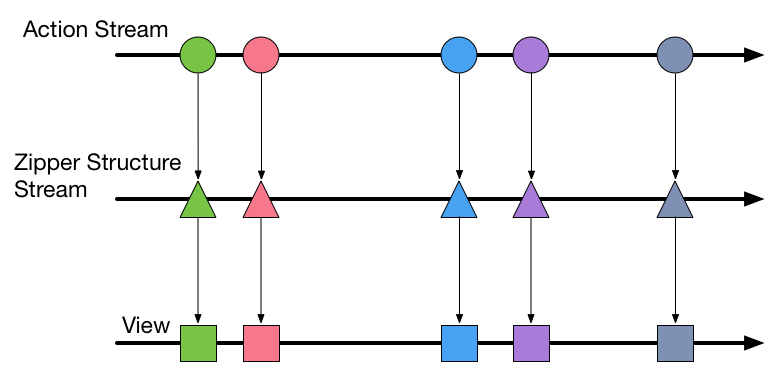
\includegraphics[width=4in]{Implementation_Diagram}
\caption{Implementation Concepts. Each Action--Zipper Structure--View combination is considered to appear ``instantaneously'' on the timeline.}
\label{fig:FRP}
\end{figure}

The key question that must be answered for any implementation strategy is how do we model a stream of actions from a user. Let us assume that these actions are chosen (using some input device, preferably, a keyboard) from some ``palette'' that never presents the user with actions that are not semantically valid, according to the action semantics defined earlier. 
%In a traditional editor, the input from the user is a stream of characters, and there are no guarantees that at any point that the program is syntactically well-formed, so the designer leaves editing as an .
%In contrast, in a structure editor, the input from the user is a stream of operations.  
As such, these actions can be considered atomic, and will always leave the program in a well-defined state. 
This insight leads us to conclude that a natural way to implement this editor would be using event-based Functional Reactive Programming~\cite{Wan:2000:FRP:349299.349331} (FRP).
Figure~\ref{fig:FRP} illustrates the concept of an FRP-based implementation of a  structure editor organized like Hazelnut.
The input from the user is a stream of actions.  Each action results in a change to the underlying model (i.e., a new Zipper Structure object is created after each input action from the user.) 
Each model change results in an updated view which is then presented to the user.  The user can then consider this new view when they choose a new action as input.

\subsection{HZ}
We explore the concepts presented in the paper in HZ, our ongoing implementation of Hazelnut.
In order to reach the widest possible audience, we decided to implement HZ in the web browser.
In order to take advantage of all the benefits of FRP, we chose to implement HZ using OCaml\footnote{https://ocaml.org/}, js\_of\_ocaml\footnote{http://ocsigen.org/js\_of\_ocaml/} and the OCaml React library\footnote{http://erratique.ch/software/react}.
Our preliminary code as well as directions for how to compile and run it can be found here: \url{https://github.com/MichaelHilton/impl-tfp16}. 
At the time of submission, HZ should very much be considered a work in progress.

A substantially simpler system that we developed while exploring the ideas that led to Hazelnut can be interacted with at the following URL:

\url{http://www.cs.cmu.edu/~comar/nestedpairs/}

\section{Related Work}\label{sec:rw}
%\subsection{Structure Editors}

Structured editing as a means to eliminate the possibility of syntax errors has a long history.  An early example is the
The Cornell Program Synthesizer~\cite{teitelbaum_cornell_1981}, first published in 1981.
The synthesizer generator~\cite{Reps:1984:SG:390010.808247} allows the user to create an attribute-grammar specification that then can be used to generate a structured editor. 
CENTAUR~\cite{Borras:1988:CS:64140.65005} produces a language specific environment from a user defined formal specification of a language.  However, none of the systems are rooted in the type-theoretic tradition.

A common application for structure editors has been for novice users. For example, 
GNOME\cite{garlan_gnome:_1984} was developed to teach programming to undergraduates.
Scratch~\cite{Resnick:2009:SP:1592761.1592779} is a structure editor targeted at children ages 8 to 16.
Touchdevelop \cite{tillmann_touchdevelop:_2011} incorporates a structure editor for programming on touch-based devices, and is used to teach high school students.
Alice~\cite{Conway:2000:ALL:332040.332481} is a 3-D programming language with an integrated structure editor for teaching novice CS undergraduate students. These are largely drag-and-drop user interfaces with a limited action model and an unclear semantics. 

Not all structure editors are for educational purposes. For example, 
mbeddr \cite{voelter_mbeddr:_2012} is an extensible C-based Programming Language and IDE (nominally, for programming embedded systems.) 
mbeddr is build on top of the commercial JetBrains MPS framework for constructing structure editors.
Another popular approach is to bring elements of structured editing into a traditional editor.
Codelets \cite{oney_codelets:_2012} uses structured editing to add interactive documentation and examples in an editor.
Barista\cite{ko_barista:_2006} allows creating of user interfaces in Java using structured editing.
Graphite~\cite{Omar:2012:ACC:2337223.2337324} allows developers to introduce structured editing interfaces called  \emph{palettes} into a text-based program editor.
These solutions all represent an incremental change from existing technologies.  However, in this paper we present a theoretical model for designing a type-theoretic structure editor from the ground up.

Perhaps the system most similar in spirit to Hazelnut is Lamdu~\cite{lamdu}. Like Hazelnut, Lambdu is both an editor and a functional language. The language is similar to Haskell, and the editor uses structure editing to enable Live Programming, where the code is always being executed as it is being written.
While Lamdu has many great features, there is no theoretical basis presented for their work -- it is a rather large body of Haskell code with an unclear (and indeed, often quite perplexing, in our experience) action model. 

Agda and Idris are two dependently typed languages that attempt to simulate a structured editor from within a rich text editor (e.g. Emacs). These systems also have notions of holes and use types to guide the user toward filling these holes. These  systems are, to our knowledge, not formally well-defined but rather exist only as part of system implementations. 





%Drag-and-drop / for novices: lots of examples, e.g. Alice and others
%
%Contemporary: Lamdu, MPS/Mbeddr, TouchDevelop
%
%Hybrid: Cyrus' active code completion paper

%\subsection{Refactoring Models}
%(Michael, can you fill this section out?)

%\subsection{Formal Editor Models}
%Need to do a search to see what else has been done...

\section{Discussion \& Conclusion}
\label{sec:future}
This paper presented Hazelnut, a type theoretic structure editor for a simply typed lambda calculus. We aim to take a principled approach to its design by formally specifying its semantics, providing strong metatheoretic guarantees, mechanizing its semantics and metatheory in Agda and implementing it using the concepts of  functional reactive programming. As of this submission, we have achieved reasonable confidence in the formal system presented above, and have transitioned our focus toward the mechanization and implementation efforts. By the time of presentation, we anticipate having complete or nearly complete versions of these. 

\subsection{Future Work}
Hazelnut is, obviously, a very limited language at its core. So the most obvious avenue for future work is to increase the expressive power of this language. Our plan is to simultaneously maintain a mechanization and implementation (following, for example, Standard ML) as we proceed, ultimately producing the first large-scale, formally verified bidirectionally typed language codesigned with a type-aware editor. It may be that certain language features are unnecessary given a sufficiently advanced type-aware structure editor, while others are practical only with editor support. We intend to use Hazelnut and derivative systems thereof as a platform for rigorously exploring such questions.

There are various aspects of the editor model that we have not yet formalized. For example, our action model does not consider how actions are actually entered using, for example, key combinations or chords. It also did not provide any specific model of how available actions will be determined for presentation to the user. In practice, we would want also to rank available actions in some reasonable manner (perhaps based on usage data gathered from other users or code repositories.)

Another research direction is in exploring how types can be used to control the presentation of expressions in the editor. For example, following our approach in a textual setting on \emph{type-specific languages} (TSLs), it should be possible to have the type that an expression is being analyzed against define alternative display forms and interaction modes \cite{TSLs}.

Finally, we did not consider any aspects of \emph{collaborative programming}, such as a packaging system, a differencing algorithm for use in a source control system, support for multiple simultaneous focii for different users, and so on. These are all interesting avenues for future work.


On the theoretical side, the notion of having one of many possible holes in a term in focus has a very strong intuitive connection
  to the proof theoretic notion of focusing \cite{Simmons11tr}. Beyond just
  the name, both seem to be a way to reduce the search space of possible
  ways to finish a derivation. We intend to explore this connection to see
  if it's coincidental or more meaningful.


  We already discussed a connection to gradual typing \cite{Siek06a}. We hope to explore this connection more thoroughly. In particular, it may be possible to better support exploratory and live programming by allowing even programs with holes in them to execute as long as those holes are only in the type portions, by deferring to the semantics given in work on gradual typing.

Looking at terms with holes in them, it's clear that there are some
  terms that ought to be identified. For example, it may be that $\hhole{\hhole{e}}$
  should be identified with $\hhole{e}$. We have not yet explored an
  equational theory for terms with holes, but intend to once our formalization
  effort is more mature.

\begin{quote}
In any case, these are but steps toward more graphical program-description
systems, for we will not forever stay confined to mere strings of symbols.

--- Marvin Minsky, Turing Award lecture
\end{quote}

%
% ---- Bibliography ----
%
% TODO
%\begin{thebibliography}{5}
\bibliographystyle{abbrv}
\bibliography{bibliography}

\clearpage
\appendix
\section{Hazelnut}
\subsection{H-Types and H-Expressions}
\subsubsection{Type Compatibility and Incompatibility}
~\\~\\
\noindent\fbox{$\tcompat{\htau}{\htau'}$}
\begin{subequations}%\label{rules:tcompat}
\begin{equation}%\label{rule:tcompat-comm}
\inferrule{
  \tcompat{\htau}{\htau'}
}{
  \tcompat{\htau'}{\htau}
}
\end{equation}
\begin{equation}%\label{rule:tcompat-hole}
\inferrule{ }{
  \tcompat{\htau}{\tehole}
}
\end{equation}
\begin{equation}%\label{rule:tcompat-num}
\inferrule{ }{
  \tcompat{\tnum}{\tnum}
}
\end{equation}
\begin{equation}%\label{rule:tcompat-arr}
\inferrule{
  \tcompat{\htau_1}{\htau_1'}\\
  \tcompat{\htau_2}{\htau_2'}
}{
  \tcompat{\tarr{\htau_1}{\htau_2}}{\tarr{\htau_1'}{\htau_2'}}
}
\end{equation}
\end{subequations}

\noindent\fbox{$\tincompat{\htau}{\htau'}$}
\begin{subequations}
  \begin{equation}
    \inferrule{
      \tincompat{\htau}{\htau'}
    }{
      \tincompat{\htau'}{\htau}
    }
  \end{equation}
  \begin{equation}
    \inferrule{ }{
      \tincompat{\tnum}{\tarr{\htau_1}{\htau_2}}
    }
  \end{equation}
  \begin{equation}
    \inferrule{
      \tincompat{\htau_1}{\htau_1'}
    }{
      \tincompat{\tarr{\htau_1}{\htau_2}}{\tarr{\htau_1'}{\htau_2'}}
    }
  \end{equation}
  \begin{equation}
    \inferrule{
      \tincompat{\htau_2}{\htau_2'}
    }{
      \tincompat{\tarr{\htau_1}{\htau_2}}{\tarr{\htau_1'}{\htau_2'}}
    }
  \end{equation}
\end{subequations}


\subsubsection{Synthesis and Analysis}
The judgements $\hsyn{\hGamma}{\hexp}{\htau}$ and $\hana{\hGamma}{\hexp}{\htau}$ are defined mutually inductively by Rules (\ref{rules:hsyn}) and Rules (\ref{rules:hana}), respectively.

\noindent\fbox{$\hsyn{\hGamma}{\hexp}{\htau}$}
\begin{subequations}\label{rules:hsyn}
\begin{equation}%\label{rule:syn-asc}
\inferrule{
  \hana{\hGamma}{\hexp}{\htau}
}{
  \hsyn{\hGamma}{\hexp : \htau}{\htau}
}
\end{equation}
\begin{equation}%\label{rule:syn-var}
\inferrule{ }{
  \hsyn{\hGamma, x : \htau}{x}{\htau}
}
\end{equation}
\begin{equation}%\label{rule:syn-ap}
\inferrule{
  \hsyn{\hGamma}{\hexp_1}{\tarr{\htau_2}{\htau}}\\
  \hana{\hGamma}{\hexp_2}{\htau_2}
}{
  \hsyn{\hGamma}{\hap{\hexp_1}{\hexp_2}}{\htau}
}
\end{equation}
\begin{equation}%\label{rule:syn-num}
\inferrule{ }{
  \hsyn{\hGamma}{\hnum{n}}{\tnum}
}
\end{equation}
\begin{equation}%\label{rule:syn-plus}
\inferrule{
  \hana{\hGamma}{\hexp_1}{\tnum}\\
  \hana{\hGamma}{\hexp_2}{\tnum}
}{
  \hsyn{\hGamma}{\hadd{\hexp_1}{\hexp_2}}{\tnum}
}
\end{equation}
\begin{equation}%\label{rule:syn-ehole}
\inferrule{ }{
  \hsyn{\hGamma}{\hehole}{\tehole}
}
\end{equation}
\begin{equation}%\label{rule:syn-hole}
\inferrule{
  \hsyn{\hGamma}{\hexp}{\htau}
}{
  \hsyn{\hGamma}{\hhole{\hexp}}{\tehole}
}
\end{equation}
\begin{equation}%\label{rule:syn-ap-2}
\inferrule{
  \hsyn{\hGamma}{\hexp_1}{\tehole}\\
  \hana{\hGamma}{\hexp_2}{\tehole}
}{
  \hsyn{\hGamma}{\hap{\hexp_1}{\hexp_2}}{\tehole}
}
\end{equation}
\end{subequations}

\noindent\fbox{$\hana{\hGamma}{\hexp}{\htau}$}
\begin{subequations}\label{rules:hana}
\begin{equation}
\inferrule{
  \hsyn{\hGamma}{\hexp}{\htau'}\\
  \tcompat{\htau}{\htau'}
}{
  \hana{\hGamma}{\hexp}{\htau}
}
\end{equation}
\begin{equation}%\label{rule:syn-lam}
\inferrule{
  \hana{\hGamma, x : \htau_1}{\hexp}{\htau_2}
}{
  \hana{\hGamma}{\hlam{x}{\hexp}}{\tarr{\htau_1}{\htau_2}}
}
\end{equation}
\end{subequations}

\subsubsection{Complete H-Types and H-Expressions}
By convention, we use the metavariable $\tau$ rather than $\htau$ for complete H-types, and $e$ rather than $\hexp$ for complete H-expressions.

~\\~\\\noindent\fbox{$\hcomplete{\tau}$} 
\begin{subequations}
\begin{equation}
\inferrule{
  \hcomplete{\tau_1}\\
  \hcomplete{\tau_2}
}{
  \hcomplete{\tarr{\tau_1}{\tau_2}}
}
\end{equation}
\begin{equation} 
\inferrule{ }{
  \hcomplete{\tnum}
}
\end{equation}
\begin{equation}
\inferrule{ }{
  \hcomplete{\tehole}
}
\end{equation}
\end{subequations}

\noindent\fbox{$\hcomplete{e}$}
\begin{subequations}
\begin{equation}
  \inferrule{
    \hcomplete{\hexp}\\
    \hcomplete{\htau}
  }{
    \hcomplete{\hexp : \htau}
  }
\end{equation}
\begin{equation}
  \inferrule{ }{
    \hcomplete{x}
  }
\end{equation}
\begin{equation}
  \inferrule{ 
    \hcomplete{\hexp}
  }{
    \hcomplete{\hlam{x}{\hexp}}
  }
\end{equation}
\begin{equation}
  \inferrule{
    \hcomplete{\hexp_1}\\
    \hcomplete{\hexp_2}
  }{
    \hcomplete{\hap{\hexp_1}{\hexp_2}}
  }
\end{equation}
\begin{equation}
  \inferrule{ }{\hcomplete{\hnum{n}}}
\end{equation}
\begin{equation}
  \inferrule{
    \hcomplete{\hexp_1}\\
    \hcomplete{\hexp_2}
  }{
    \hcomplete{\hadd{\hexp_1}{\hexp_2}}
  }
\end{equation}
\begin{equation}
  \inferrule{ }{\hcomplete{\hehole}}
\end{equation}
\begin{equation}
  \inferrule{
    \hcomplete{\hexp}
  }{
    \hcomplete{\hhole{\hexp}}
  }
\end{equation}
\end{subequations}

\subsection{Z-Types and Z-Expressions}
\subsubsection{Type Focus Erasure}~\\~\\
\noindent\fbox{$\removeSel{\ztau}=\htau$} is a metafunction defined as follows:
\begin{subequations}
\begin{align}
%\removeSel{(\zlsel{\htau})} & = \htau\\
\removeSel{(\zwsel{\htau})} & = \htau\\
%\removeSel{(\zrsel{\htau})} & = \htau\\
\removeSel{(\tarr{\ztau}{\htau})} & = \tarr{\removeSel{\ztau}}{\htau}\\
\removeSel{(\tarr{\htau}{\ztau})} & = \tarr{\htau}{\removeSel{\ztau}}
\end{align}
\end{subequations}

\subsubsection{Expression Focus Erasure}~\\~\\
\noindent\fbox{$\removeSel{\zexp}=\hexp$} is a metafunction defined as follows:
\begin{subequations}
\begin{align}
%\removeSel{(\zlsel{\hexp})} & = \hexp\\
\removeSel{(\zwsel{\hexp})} & = \hexp\\
%\removeSel{(\zrsel{\hexp})} & = \hexp\\
\removeSel{(\zexp : \htau)} & = \removeSel{\zexp} : \htau\\
\removeSel{(\hexp : \ztau)} & = \hexp : \removeSel{\ztau}\\
\removeSel{(\hlam{x}{\zexp})} & = \hlam{x}{\removeSel{\zexp}}\\
\removeSel{(\hap{\zexp}{\hexp})} & = \hap{\removeSel{\zexp}}{\hexp}\\
\removeSel{(\hap{\hexp}{\zexp})} & = \hap{\hexp}{\removeSel{\zexp}}\\
\removeSel{(\hadd{\zexp}{\hexp})} & = \hadd{\removeSel{\zexp}}{\hexp}\\
\removeSel{(\hadd{\hexp}{\zexp})} & = \hadd{\hexp}{\removeSel{\zexp}}\\
\removeSel{\hhole{\zexp}} &= \hhole{\removeSel{\zexp}}
\end{align}
\end{subequations}
\subsection{Action Model}
\subsubsection{Type Actions}~\\~\\
\noindent\fbox{$\performTyp{\ztau}{\alpha}{\ztau'}$}
\paragraph{Type Movement}
\begin{subequations}
\begin{equation}
  \inferrule{ }{
    \performTyp{
      \zwsel{\tarr{\htau_1}{\htau_2}}
    }{
      \aMove{\dChild}
    }{
      \tarr{\zwsel{\htau_1}}{\htau_2}
    }
  }
\end{equation}
\begin{equation}
  \inferrule{ }{
    \performTyp{
      \tarr{\zwsel{\htau_1}}{\htau_2}
    }{
      \aMove{\dParent}
    }{
      \zwsel{\tarr{\htau_1}{\htau_2}}
    }
  }
\end{equation}
\begin{equation}
  \inferrule{ }{
    \performTyp{
      \tarr{{\htau_1}}{\zwsel{\htau_2}}
    }{
      \aMove{\dParent}
    }{
      \zwsel{\tarr{\htau_1}{\htau_2}}
    }
  }
\end{equation}
\begin{equation}
  \inferrule{ }{
    \performTyp{
      \tarr{\zwsel{\htau_1}}{{\htau_2}}
    }{
      \aMove{\dNext}
    }{
      {\tarr{\htau_1}{\zwsel{\htau_2}}}
    }
  }
\end{equation}
\begin{equation}
  \inferrule{ }{
    \performTyp{
      \tarr{{\htau_1}}{\zwsel{\htau_2}}
    }{
      \aMove{\dPrev}
    }{
      {\tarr{\zwsel{\htau_1}}{{\htau_2}}}
    }
  }
\end{equation}
\begin{equation}
\inferrule{
  \performTyp{
    \ztau
  }{
    \aMove{\delta}
  }{
    \ztau'
  }
}{
  \performTyp{
    \tarr{\ztau}{\htau}
  }{
    \aMove{\delta}
  }{
    \tarr{\ztau'}{\htau}
  }
}
\end{equation}
\begin{equation}
  \inferrule{
    \performTyp{
      \ztau
    }{
      \aMove{\delta}
    }{
      \ztau'
    }
  }{
    \performTyp{
      \tarr{\htau}{\ztau}
    }{
      \aMove{\delta}
    }{
      \tarr{\htau}{\ztau}
    }
  }
\end{equation}

\paragraph{Type Deletion}
\begin{equation}
  \inferrule{ }{
    \performTyp{
      \zwsel{\htau}
    }{
      \aDel
    }{
      \zwsel{\tehole}
    }
  }
\end{equation}

\paragraph{Type Construction}
\begin{equation}
    %\label{r:contarr}
  \inferrule{ }{
    \performTyp{
      \zwsel{\htau}
    }{
      \aConstruct{\farr}
    }{
      \tarr{\htau}{\zwsel{\tehole}}
    }
  }
\end{equation}

  \begin{equation}
    %\label{r:contnum}
  \inferrule{ }{
    \performTyp{
      \zwsel{\tehole}
    }{
      \aConstruct{\fnum}
    }{
      \zwsel{\tnum}
    }
  }
\end{equation}


\paragraph{Zipper Cases}
  \begin{equation}
    %\label{r:contarrL}
  \inferrule{
    \performTyp{\ztau}{\alpha}{\ztau'}
  }{
    \performTyp{
      \tarr{\ztau}{\htau}
    }{
      \alpha
    }{
      \tarr{\ztau'}{\htau}
    }
  }
\end{equation}
  \begin{equation}
    %\label{r:contarrR}
  \inferrule{
    \performTyp{\ztau}{\alpha}{\ztau'}
  }{
    \performTyp{
      \tarr{\htau}{\ztau}
    }{
      \alpha
    }{
      \tarr{\htau}{\ztau'}
    }
  }
\end{equation}
\end{subequations}

\subsubsection{Expression Movement Actions}~\\~\\
\noindent\fbox{$\performMove{\zexp}{\aMove{\delta}}{\zexp'}$}

\begin{subequations}
\paragraph{Ascription}

\begin{equation}
  \inferrule{ }{
    \performMove{
      \zwsel{\hexp : \htau}
    }{
      \aMove{\dChild}
    }{
      \zwsel{\hexp} : \htau
    }
  }
\end{equation}
\begin{equation}
  \inferrule{ }{
    \performMove{
      \zwsel{\hexp} : \htau
    }{
      \aMove{\dParent}
    }{
      \zwsel{\hexp : \htau}
    }
  }
\end{equation}
\begin{equation}
  \inferrule{ }{
    \performMove{
      \hexp : \zwsel{\htau}
    }{
      \aMove{\dParent}
    }{
      \zwsel{\hexp : \htau}
    }
  }
\end{equation}
\begin{equation}
  \inferrule{ }{
    \performMove{
      \zwsel{\hexp} : \htau
    }{
      \aMove{\dNext}
    }{
      \hexp : \zwsel{\htau}
    }
  }
\end{equation}
\begin{equation}
  \inferrule{ }{
    \performMove{
      \hexp : \zwsel{\htau}
    }{
      \aMove{\dPrev}
    }{
      \zwsel{\hexp} : \htau
    }
  }
\end{equation}
\begin{equation}
\inferrule{
  \performMove{
    \zexp
  }{
    \aMove{\delta}
  }{
    \zexp'
  }
}{
  \performMove{
    \zexp : \htau
  }{
    \aMove{\delta}
  }{
    \zexp' : \htau
  }
}
\end{equation}
\begin{equation}
  \inferrule{
    \performMove{
      \ztau
    }{
      \aMove{\delta}
    }{
      \ztau'
    }
  }{
    \performMove{
      \hexp : \ztau
    }{
      \aMove{\delta}
    }{
      \hexp : \ztau'
    }
  }
\end{equation}

\paragraph{Lambda}
\begin{equation}
\inferrule{ }{
  \performMove{
    \zwsel{\hlam{x}{\hexp}}
  }{
    \aMove{\dChild}
  }{
    \hlam{x}{\zwsel{\hexp}}
  }
}
\end{equation}
\begin{equation}
  \inferrule{ }{
    \performMove{
      \hlam{x}{\zwsel{\hexp}}
    }{
      \aMove{\dParent}
    }{
      \zwsel{\hlam{x}{\hexp}}
    }
  }
\end{equation}
TODO: zipper cases?
\paragraph{Application}
\begin{equation}
  \inferrule{ }{
    \performMove{
      \zwsel{\hap{\hexp_1}{\hexp_2}}
    }{
      \aMove{\dChild}
    }{
      \hap{\zwsel{\hexp_1}}{\hexp_2}
    }
  }
\end{equation}
\begin{equation}
  \inferrule{ }{
    \performMove{
      \hap{\zwsel{\hexp_1}}{\hexp_2}
    }{
      \aMove{\dParent}
    }{
      \zwsel{\hap{\hexp_1}{\hexp_2}}
    }
  }
\end{equation}
\begin{equation}
  \inferrule{ }{
    \performMove{
      \hap{{\hexp_1}}{\zwsel{\hexp_2}}
    }{
      \aMove{\dParent}
    }{
      \zwsel{\hap{\hexp_1}{\hexp_2}}
    }
  }
\end{equation}
\begin{equation}
  \inferrule{ }{
    \performMove{
      \hap{\zwsel{\hexp_1}}{\hexp_2}
    }{
      \aMove{\dNext}
    }{
      \hap{\hexp_1}{\zwsel{\hexp_2}}
    }
  }
\end{equation}
\begin{equation}
  \inferrule{ }{
    \performMove{
      \hap{\hexp_1}{\zwsel{\hexp_2}}
    }{
      \aMove{\dPrev}
    }{
      \hap{\zwsel{\hexp_1}}{\hexp_2}
    }
  }
\end{equation}
TODO: Zipper cases?

\paragraph{Plus}
\begin{equation}
  \inferrule{ }{
    \performMove{
      \zwsel{\hadd{\hexp_1}{\hexp_2}}
    }{
      \aMove{\dChild}
    }{
      \hadd{\zwsel{\hexp_1}}{\hexp_2}
    }
  }
\end{equation}
\begin{equation}
  \inferrule{ }{
    \performMove{
      \hadd{\zwsel{\hexp_1}}{\hexp_2}
    }{
      \aMove{\dParent}
    }{
      \zwsel{\hadd{\hexp_1}{\hexp_2}}
    }
  }
\end{equation}
\begin{equation}
  \inferrule{ }{
    \performMove{
      \hadd{{\hexp_1}}{\zwsel{\hexp_2}}
    }{
      \aMove{\dParent}
    }{
      \zwsel{\hadd{\hexp_1}{\hexp_2}}
    }
  }
\end{equation}
\begin{equation}
  \inferrule{ }{
    \performMove{
      \hadd{\zwsel{\hexp_1}}{\hexp_2}
    }{
      \aMove{\dNext}
    }{
      \hadd{\hexp_1}{\zwsel{\hexp_2}}
    }
  }
\end{equation}
\begin{equation}
  \inferrule{ }{
    \performMove{
      \hadd{\hexp_1}{\zwsel{\hexp_2}}
    }{
      \aMove{\dPrev}
    }{
      \hadd{\zwsel{\hexp_1}}{\hexp_2}
    }
  }
\end{equation}
TODO: Zipper cases?

\paragraph{Non-Empty Hole}
\begin{equation}
\inferrule{ }{
  \performMove{
    \zwsel{\hhole{\hexp}}
  }{
    \aMove{\dChild}
  }{
    \hhole{\zwsel{\hexp}}
  }
}
\end{equation}
\begin{equation}
  \inferrule{ }{
    \performMove{
      \hhole{\zwsel{\hexp}}
    }{
      \aMove{\dParent}
    }{
      \zwsel{\hhole{\hexp}}
    }
  }
\end{equation}
TODO: Zipper case?

\end{subequations}
\subsubsection{Synthetic Expression Actions}~\\~\\
\noindent\fbox{$\performSyn{\hGamma}{\zexp}{\htau}{\alpha}{\zexp'}{\htau'}$}

\begin{subequations}
\paragraph{Movement} 
\begin{equation}
\inferrule{
  \performMove{\zexp}{\aMove{\delta}}{\zexp'}
}{
  \performSyn{\hGamma}{\zexp}{\htau}{\aMove{\delta}}{\zexp'}{\htau}
}
\end{equation}

\paragraph{Deletion} 
\begin{equation}
  \inferrule{ }{
    \performSyn{\hGamma}{\zwsel{\hexp}}{\htau}{\aDel}{\zwsel{\hehole}}{\tehole}
  }
\end{equation}

\paragraph{Construction}
\begin{equation}
  \inferrule{ }{
    \performSyn{\hGamma}{\zwsel{\hexp}}{\htau}{\aConstruct{\fasc}}{\hexp : \zwsel{\htau}}{\htau}
  }
\end{equation} 

\begin{equation}
  \inferrule{ }{
    \performSyn{\hGamma, x : \htau}{\zwsel{\hehole}}{\tehole}{\aConstruct{\fvar{x}}}{\zwsel{x}}{\htau}
  }
\end{equation}

\begin{equation}
  \inferrule{ }{
    \performSyn
      {\hGamma}
      {\zwsel{\hehole}}
      {\tehole}
      {\aConstruct{\flam{x}}}
      {\hlam{x}{\hehole} : \tarr{\zwsel{\tehole}}{\tehole}}
      {\tarr{\tehole}{\tehole}}
  }
\end{equation}

\begin{equation}
  \inferrule{ }{
    \performSyn
      {\hGamma}
      {\zwsel{\hexp}}
      {\tarr{\htau_1}{\htau_2}}
      {\aConstruct{\fap}}
      {\hap{\hexp}{\zwsel{\hehole}}}
      {\htau_2}
  }
\end{equation}

\begin{equation}
  \inferrule{ }{
    \performSyn
      {\hGamma}
      {\zwsel{\hexp}}
      {\tehole}
      {\aConstruct{\fap}}
      {\hap{\hexp}{\zwsel{\hehole}}}
      {\tehole}
  }
\end{equation}

\begin{equation}
  \inferrule{
    \tincompat{\htau}{\tarr{\tehole}{\tehole}}
  }{
    \performSyn
      {\hGamma}
      {\zwsel{\hexp}}
      {\htau}
      {\aConstruct{\fap}}
      {\hap{\hhole{\hexp}}{\zwsel{\hehole}}}
      {\tehole}
  }
\end{equation}

\begin{equation}
  \inferrule{ }{
    \performSyn
      {\hGamma}
      {\zwsel{\hexp}}
      {\htau}
      {\aConstruct{\farg}}
      {\hap{\zwsel{\hehole}}{\hexp}}
      {\tehole}
  }
\end{equation}

\begin{equation}
  \inferrule{ }{
    \performSyn
      {\hGamma}
      {\zwsel{\hehole}}
      {\tehole}
      {\aConstruct{\fnumlit{n}}}
      {\zwsel{\hnum{n}}}
      {\tnum}
  }
\end{equation}

\begin{equation}
  \inferrule{
    \tcompat{\htau}{\tnum}
  }{
    \performSyn
      {\hGamma}
      {\zwsel{\hexp}}
      {\htau}
      {\aConstruct{\fplus}}
      {\hadd{\hexp}{\zwsel{\hehole}}}
      {\tnum}
  }
\end{equation}

\begin{equation}
  \inferrule{
    \tincompat{\htau}{\tnum}
  }{
    \performSyn
      {\hGamma}
      {\zwsel{\hexp}}
      {\htau}
      {\aConstruct{\fplus}}
      {\hadd{\hhole{\hexp}}{\zwsel{\hehole}}}
      {\tnum}
  }
\end{equation}

\paragraph{Finishing}
  \begin{equation}
    \label{r:finishana}
  \inferrule{
    \hsyn{\hGamma}{\hexp}{\htau'}
  }{
    \performSyn
      {\hGamma}
      {\zwsel{\hhole{\hexp}}}
      {\tehole}
      {\aFinish}
      {\zwsel{\hexp}}
      {\htau'}
  }
\end{equation}


\paragraph{Zipper Cases} e
\end{subequations}

\subsubsection{Analytic Expression Actions}~\\~\\
\noindent\fbox{$\performAna{\hGamma}{\zexp}{\htau}{\alpha}{\zexp'}$}
\begin{subequations}
\paragraph{Subsumption} 
\begin{equation}
  \inferrule{
    \performSyn{\hGamma}{\zexp}{\htau'}{\alpha}{\zexp'}{\htau''}\\
    \tcompat{\htau}{\htau''}
  }{
    \performAna{\hGamma}{\zexp}{\htau}{\alpha}{\zexp'}
  }
\end{equation}

TODO: require synthesis as premise? 

\paragraph{Movement}
\begin{equation}
  \inferrule{
  \performMove{\zexp}{\aMove{\delta}}{\zexp'}
}{
  \performAna{\hGamma}{\zexp}{\htau}{\aMove{\delta}}{\zexp'}
}
\end{equation} 

\paragraph{Deletion}
\begin{equation}
  \inferrule{ }{
    \performAna{\hGamma}{\zwsel{\hexp}}{\htau}{\aDel}{\zwsel{\hehole}}
  }
\end{equation}

\paragraph{Construction}
\begin{equation}
  \inferrule{ }{
    \performAna{\hGamma}{\zwsel{\hexp}}{\htau}{\aConstruct{\fasc}}{\hexp : \zwsel{\htau}}
  }
\end{equation} 

\begin{equation}
  \inferrule{
    \tincompat{\htau}{\htau'}
  }{
    \performAna{\hGamma, x : \htau'}{\zwsel{\hehole}}{\htau}{\aConstruct{\fvar{x}}}{\hhole{\zwsel{x}}}
  }
\end{equation}

\begin{equation}
  \inferrule{ }{
    \performAna
      {\hGamma}
      {\zwsel{\hehole}}
      {\tarr{\htau_1}{\htau_2}}
      {\aConstruct{\flam{x}}}
      {\hlam{x}{\zwsel{\hehole}}}
  }
\end{equation}

\begin{equation}
  \inferrule{
    \tincompat{\htau}{\tarr{\tehole}{\tehole}}
  }{
    \performAna
      {\hGamma}
      {\zwsel{\hehole}}
      {\htau}
      {\aConstruct{\flam{x}}}
      {\hhole{
        \hlam{x}{\hehole} : \tarr{\zwsel{\tehole}}{\tehole}
      }}
  }
\end{equation}
\begin{equation}
  \inferrule[test]{
    \tincompat{\htau}{\tnum}
  }{
    \performAna
      {\hGamma}
      {\zwsel{\hehole}}
      {\htau}
      {\aConstruct{\fnumlit{n}}}
      {\hhole{\zwsel{\hnum{n}}}}
  }
\end{equation}
\paragraph{Finishing} 
\begin{equation}
  \inferrule{
    \hana{\hGamma}{\hexp}{\htau}
  }{
    \performAna
      {\hGamma}
      {\zwsel{\hhole{\hexp}}}
      {\htau}
      {\aFinish}
      {\zwsel{\hexp}}
  }
\end{equation}

\paragraph{Zipper Cases} e

\end{subequations}
\end{document}
